\chapter{Análisis y simulaciones de prueba}\label{cap.pruebas}

La naturaleza de este proyecto no solo contempla la implementación de un código que sea capaz de realizar simulaciones de entornos 5G, sino que también está orientado a ofrecer resultados de simulaciones realizadas, y orientaciones sobre cómo efectuar simulaciones apropiadas para el paradigma de 5G y \acs{hetnet}s.

Por ello, este capítulo está dedicado a la exposición de una serie de simulaciones realizadas a través de 5Gneralife, con la finalidad de evaluar el comportamiento de las redes 5G en distintas condiciones, a través de la variación progresiva de parámetros, así como valorar el rendimiento del mismo, tiempos de ejecución y recursos computacionales consumidos.

Para comenzar, se realizará en una primera sección una descripción de los detalles que se deben tener en cuenta y los parámetros recomendados a la hora de realizar una simulación realista. A continuación, se realizará una demostración de un entorno realista siguiendo dichas pautas. Por último, se llevarán a cabo un conjunto de simulaciones experimentales para evaluar cambios en el comportamiento de escenarios 5G.

\section{Estándar propuesto}

Aunque todas las implementaciones que se han llevado a cabo para la elaboración de este simulador han sido orientadas hacia la funcionalidad de 5G, no hay que olvidar que el software en el que se basa, \textit{QuaDRiGa}, fue diseñado con vistas en LTE, con posterior adaptación a 5G. Esto supone que la elección de parámetros deben ser consecuentes con el escenario deseado y, por tanto, hay que prestar especial atención a ciertos detalles de la naturaleza de 5G.

Por ello, está sección está dedicada a recopilar los detalles que se deben tener en cuenta a la hora de realizar simulaciones que se esperan que sean realistas, junto a parámetros o rango de parámetros recomendados para que el escenario sea lo más ajustado posible a 5G.

A continuación, se detalla un listado de consideraciones:
\begin{itemize}
    \item Las macro-celdas se encuentran para auxiliar a las micro-celdas y no al revés, como se concebía en LTE. Esto implica que se debe desplegar un entorno en el que se espera que la mayor concentración de usuarios se den en los enlaces hacia micro-celdas, por lo que es necesario dimensionarlas de forma que el enlace por SINR -o, en su defecto, por distancia- sea favorable siempre en la capa de micro-celdas con respecto a la capa de macro-celdas. Por ello, se propone que la distancia entre micro-celdas sea aproximadamente la mitad que la distancia entre macro-celdas establecida, a la vez que la potencia de transmisión recomendada sea de 40 dBm para macro-celdas y 27 dBm para micro-celdas. Con esta configuración se han obtenido unos resultados óptimos de cobertura.
    \item Un escenario con una relación cobertura-proporción de número de elementos desplegados razonable es la de despliegue de 7 macro-celdas y 19 micro-celdas para ofrecer una cobertura optimizada de acuerdo a la separación entre sus centros establecida anteriormente.
    \item El modelo de ruido térmico típico para 5G se suele especificar con una densidad espectral de $4.04·10^{-21}$ W/Hz \cite{ruido}.
    \item La probabilidad de encontrar visión directa según el reporte técnico de 3GPP 38.901 se encuentra en 20\%, correspondiendo un 80\% para el caso de NLOS de acuerdo a los estudios presentados en su última versión.
    \item La frecuencia estándar para macro-celdas urbanas es de aproximadamente 2,6 GHz, mientras que para micro-celdas sería de 20 GHz.
    \item No es realista que todos los usuarios realicen una trayectoria sin final. Por este motivo y también para evitar simulaciones de larga duración, lo razonable es que una persona recorra una media de 2 km mientras se desplaza por la calle.
\end{itemize}

Establecidas estas recomendaciones, comentar que \textit{5Gneralife} permite cualquier configuración en la medida de lo razonable y que dependiendo del número de usuarios, esta simulación puede llevarse a cabo o no, debido a que una gran cantidad de usuarios puede llegar a consumir todos los recursos de memoria y aumenta considerablemente el tiempo de ejecución.

\section{Estudio completo de una sola simulación}

En primer lugar para ilustrar el potencial del simulador, se ha efectuado una simulación consistente en un entorno con 100 usuarios en movimiento. Cada usuario recorre 250 metros a una velocidad de un metro por segundo y se encuentra utilizando un terminal móvil con interfaz dual compatible con macro-celdas y micro-celdas.

La frecuencia de las celdas son de 2,6 GHz para el caso de las macro-celdas y de 20 GHz para micro-celdas. Además, los centros de las macro-celdas se encuentran separados entre sí por 3 km, mientras que los de las micro-celdas están separados por 1,3 km. La potencia de transmisión son de 40 dBm y 27 dBm para macro-celdas y micro-celdas respectivamente.

Se ha adoptado un ancho de banda de 100 MHz por celda y un ruido térmico con una densidad espectral de $4.04·10^{-21}$ W/Hz. 

Se puede ver una representación gráfica del resultado final en la figura \ref{fig:simulacion_completa_entorno}:

\begin{figure}[h!]
	\centering
    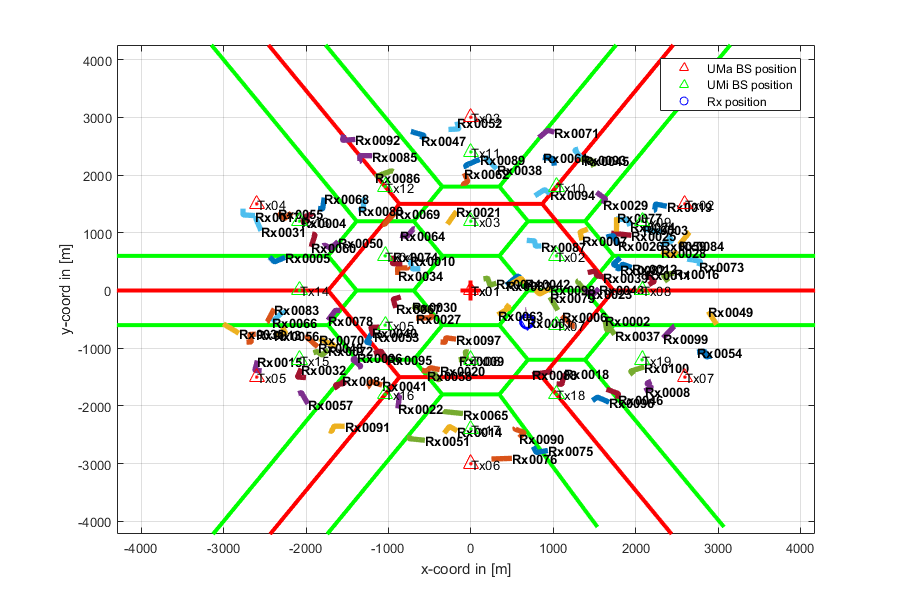
\includegraphics[width=0.8\linewidth]{imagenes/6_2_entorno.png}
	\caption{Visualización del entorno simulado.}
	\label{fig:simulacion_completa_entorno}
\end{figure}

Esta simulación ha tomado un tiempo de ejecución de 5 horas, 28 minutos y 3 segundos con el equipo descrito en la sección de recursos. Para la simulación se ha llegado a requerir un máximo de 3 GB de memoria RAM, y la media de utilización de CPU ha sido del 33\% a lo largo de toda su ejecución. Para el almacenamiento de los datos generados se han necesitado 17,80 MB de espacio. Se estima que si esta simulación hubiese contado con un recorrido por parte de los usuarios de 1 km, esta habría tardado aproximadamente 27 horas.

Para mostrar unos resultados significativos, se ha considerado comparar las variables de SINR y capacidad de los cuatro primeros receptores para las dos capas de simulación en un total de cuatro figuras.

En las dos primeras, Figura \ref{fig:simulacion_completa_cap_uma} y Figura \ref{fig:simulacion_completa_cap_umi} se puede comparar la capacidad de salida para dichos usuarios en el caso de la capa de macro-celdas y de micro-celdas respectivamente:

\begin{figure}[h!]
	\centering
    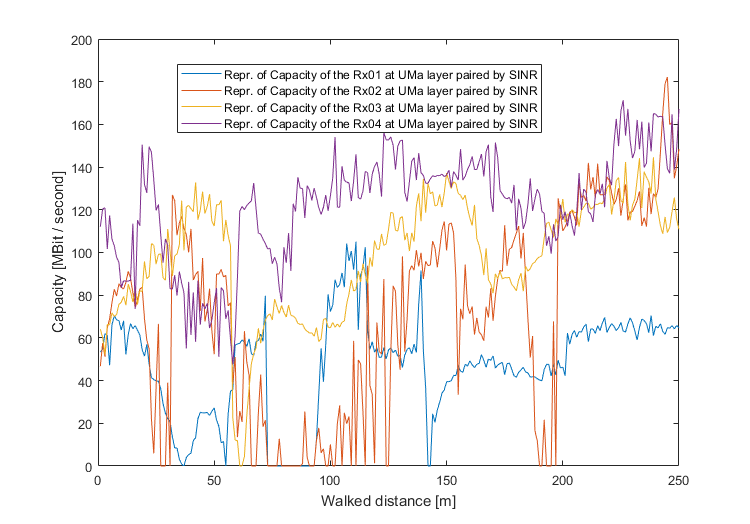
\includegraphics[width=0.8\linewidth]{imagenes/6_2_capacidad_uma.png}
	\caption{Capacidad de canal para los primeros cuatro usuarios en la capa de macro-celda.}
	\label{fig:simulacion_completa_cap_uma}
\end{figure}

\begin{figure}[h!]
	\centering
    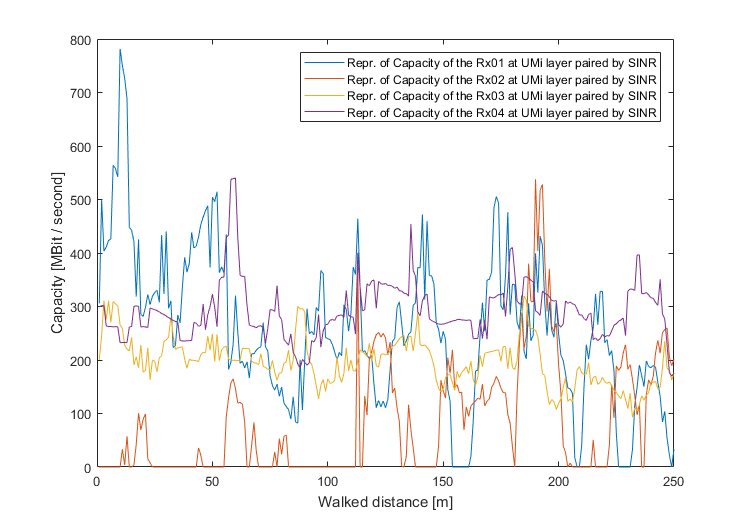
\includegraphics[width=0.8\linewidth]{imagenes/6_2_capacidad_umi.png}
	\caption{Capacidad de canal para los primeros cuatro usuarios en la capa de micro-celda.}
	\label{fig:simulacion_completa_cap_umi}
\end{figure}

Se observa una capacidad asignada significativamente mayor para el caso de micro-celdas. Este resultado es de esperar si se tiene en cuenta que el número de usuarios conectados en la capa de micro-celdas a una misma estación base siempre es menor que en el caso de la capa de macro-celdas, por lo que el ancho de banda es repartido entre menor cantidad de usuarios.

\begin{figure}[h!]
	\centering
    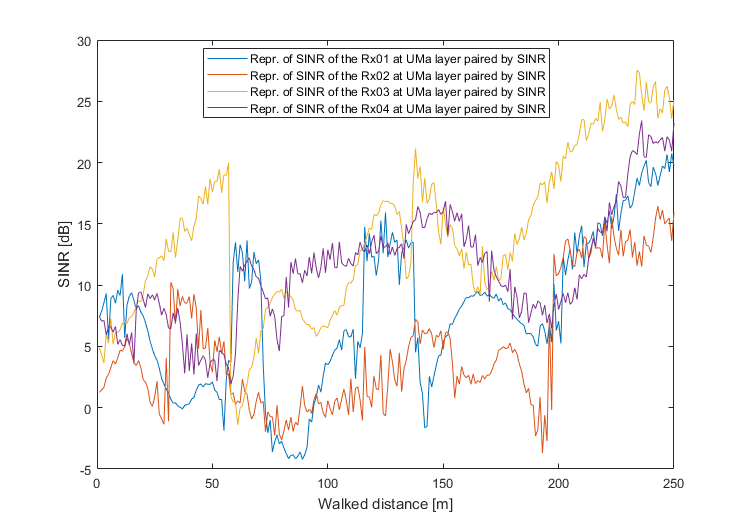
\includegraphics[width=0.8\linewidth]{imagenes/6_2_sinr_uma.png}
	\caption{SINR para los primeros cuatro usuarios en la capa de macro-celda.}
	\label{fig:simulacion_completa_sinr_uma}
\end{figure}

\begin{figure}[h!]
	\centering
    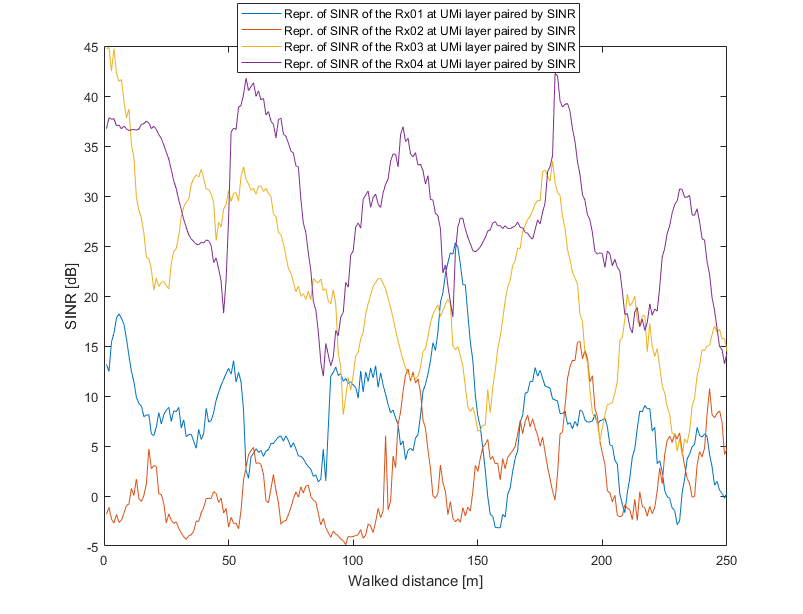
\includegraphics[width=0.8\linewidth]{imagenes/6_2_sinr_umi.png}
	\caption{SINR para los primeros cuatro usuarios en la capa de micro-celda.}
	\label{fig:simulacion_completa_sinr_umi}
\end{figure}

Por otro lado, en cuanto a SINR, como se aprecia en las Figuras \ref{fig:simulacion_completa_sinr_uma} y \ref{fig:simulacion_completa_sinr_umi}, aunque los resultado se decantan por ser ligeramente propicios en el caso de las micro-celdas, la diferencia no es sumamente relevante. Esto demuestra que el factor que hacía que la capacidad de canal asignada fuera mayor en micro-celdas era el reparto de usuarios en las celdas. Esto justifica la existencia de las micro-celdas en generaciones avanzadas de radio-comunicaciones, ya que su funcionalidad es precisamente descargar de usuarios a las celdas más grandes.

Del mismo modo, es posible comparar los dos criterios de emparejamiento disponibles a través de la comparativa entre la capacidad en ambos casos. Para ello, se ha representado en una misma figura la evolución de la capacidad en los dos casos de emparejamiento, como aparece en la Figura \ref{fig:simulacion_completa_sinr_umi_vs_cercano}.

\begin{figure}[h!]
	\centering
    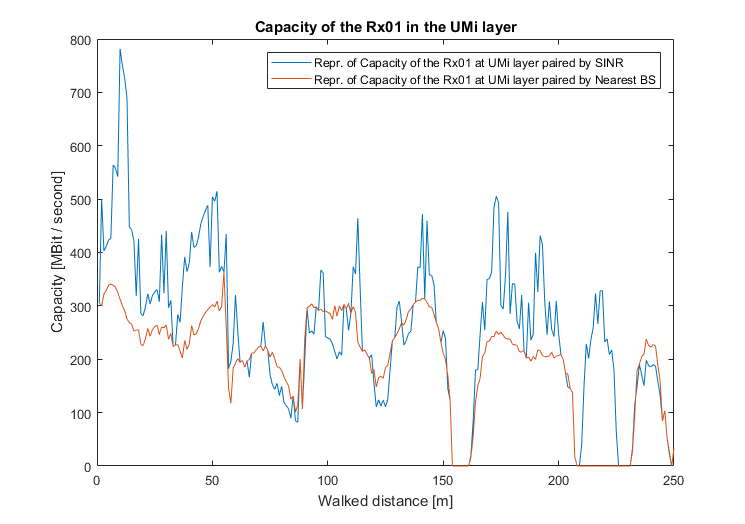
\includegraphics[width=0.8\linewidth]{imagenes/6_2_capacidad_umi_sinr_vs_cercano.png}
	\caption{Comparativa de la capacidad del primer receptor para los dos criterios de emparejamiento.}
	\label{fig:simulacion_completa_sinr_umi_vs_cercano}
\end{figure}

En ella se muestra que, por lo general, el criterio de emparejamiento de mayor SINR es por lo general mejor. Sin embargo, hay tramos en los que ocurren excepciones y que demuestran que hay ocasiones en las que es mejor para el rendimiento de la red asignar los usuarios a otras celdas que no sean las óptimas, ya que en casos de congestión existirá saturación.

Por último, podría resultar también interesante consultar cómo evoluciona la capacidad asignada de acuerdo con la SINR recibida. En la Figura \ref{fig:simulacion_completa_sinr_uma_vs_capacidad} se muestra a la vez la SINR y la capacidad del primer usuario a lo largo de su recorrido.

\begin{figure}[h!]
	\centering
    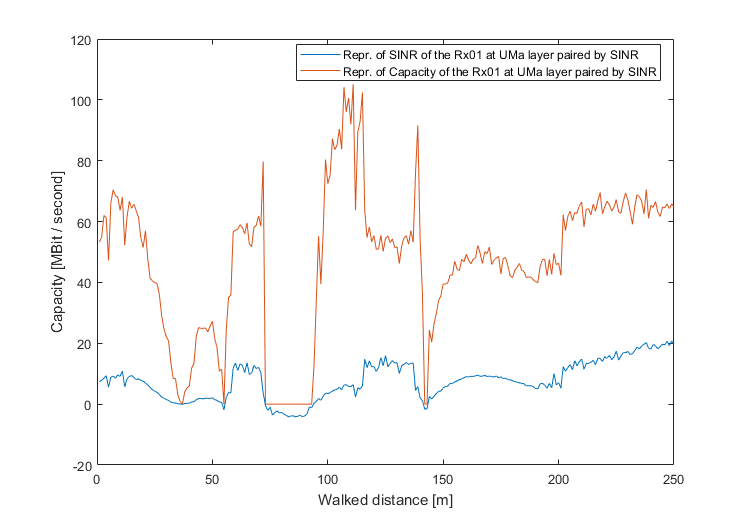
\includegraphics[width=0.8\linewidth]{imagenes/6_2_capacidad_vs_sinr_uma.png}
	\caption{Evolución de la SINR y de la capacidad para el primer usuario.}
	\label{fig:simulacion_completa_sinr_uma_vs_capacidad}
\end{figure}

De los datos de simulación generados se puede extraer con una evaluación breve que el sistema se comporta tal y como se esperaba, con resultados proporcionados, un comportamiento realista en cuanto a rendimiento de la red se refiere y con una completa cohesión entre las salidas.

\section{Comparativa entre simulaciones}

No solamente es interesante el estudio de un escenario complejo de simulación como el anterior, sino que también resulta conveniente realizar las oportunas pruebas para estudiar cómo cambia el comportamiento de las variables de salida al alterar diversos parámetros de simulación.

Por ello, como último conjunto de pruebas, se han realizado tres estudios independientes con la finalidad de evaluar la repercusión en ambas camas de simulación para tres parámetros distintos: frecuencia, potencia de transmisión y separación entre centros de celdas.

Para las simulaciones se ha establecido un recorrido fijo para un único receptor, el cual recorre 1.000 metros a lo largo de un entorno con 7 macro-celdas y 19 micro-celdas. Se ha fijado el ancho de banda de cada celda a 100 MHz y el ruido con una densidad de $4.04·10^{-21}$ W/Hz. En concreto, el recorrido que realiza el receptor es el mostrado en la Figura \ref{fig:recorrido_pruebas}.

\begin{figure}[h!]
	\centering
    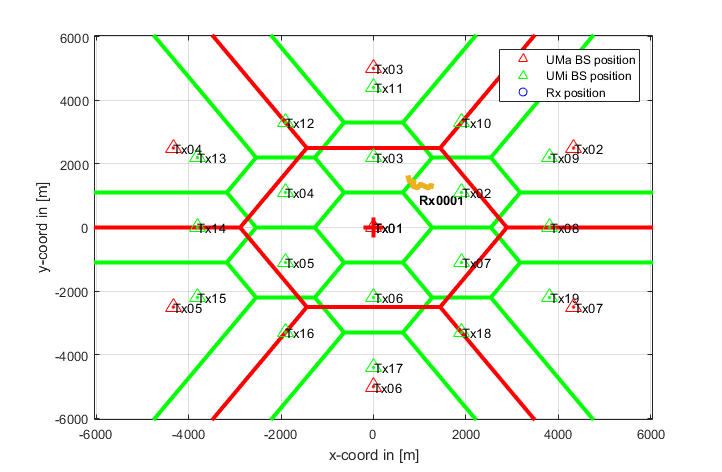
\includegraphics[width=0.8\linewidth]{imagenes/representacion_pruebas_entorno.png}
	\caption{Entorno de simulación de pruebas con el recorrido del único receptor.}
	\label{fig:recorrido_pruebas}
\end{figure}

En dicha representación se puede observar que el receptor se encuentra en una posición a poca distancia del centro de la primera celda en el caso de macro-celdas, mientras que el escenario para las micro-celdas es algo menos propicio, puesto que se aprecia que el receptor pasa de una celda a otra, encontrándose en todo momento en la frontera entre la celda 2 y la celda 3 de dicha capa, por lo que es de esperar que las comunicaciones en la capa de celdas no sean las óptimas en casi todas las simulaciones.

Aunque los resultados pueden otorgar información de cómo afecta al entorno, este número de simulaciones no es suficiente para resultar concluyente, puesto que las condiciones tienen una componente aleatoria que puede propiciar las interferencias en un determinado caso entre otros aspectos conflictivos. La mejor metodología a seguir sería repetir la simulación de la anterior sección realizando un barrido paramétrico para cada una de las variables, y recopilando información sobre los valores medios de salida para todos los receptores. Sin embargo, esta labor podría llevar miles de horas con un solo ordenador como el que se ha utilizado, por lo que se ha optado por esta simplificación que puede resultar de igual modo significativa.

\subsection{Evolución de la frecuencia}

El primer parámetro que se variará para evaluar el comportamiento del escenario es la frecuencia. Para realizar el experimento, se han diseñado tres casos en los que únicamente varía la frecuencia asignada a los dos tipos de celda en cada uno de ellos, manteniendo estático el resto de parámetros.

En cuanto a los parámetros estáticos, se ha diseñado una simulación con un receptor que recorre 1.000 metros. La capa de macro-celdas está compuesta por 7 celdas, mientras que la de las micro-celdas, está compuesta por 19, con una separación entre sus centros de 5 km y 2,2 km respectivamente. Se ha mantenido el ruido fijo con una densidad espectral de potencia de $4,04·10^{-21}$ W/Hz, y un ancho de banda de 100 MHz para ambas capas. La potencia de transmisión se ha fijado a 40 dBm para macro-celdas y 27 dBm para micro-celdas.

En primer lugar, se ha realizado una simulación inicial con una frecuencia que se estima como mínima, puesto que se ha asignado 1 GHz para macro-celdas y 6 GHz para las micro-celdas. Para este caso, se ha representado la capacidad obtenida por el receptor en el caso de conexión a macro-celdas en la Figura \ref{fig:simulacion_freq_min_uma} y en el caso de conexión a micro-celdas en la Figura \ref{fig:simulacion_freq_min_umi}, ambas para el caso de emparejamiento de la estación base con mayor SINR.

Esta simulación ha tomado un total de 21 minutos y 44 segundos para su ejecución, obteniendo un pico de utilización de memoria de 1 GB y ocupando 7,88 MB de almacenamiento al ser guardada en el disco duro.

\begin{figure}[h!]
	\centering
    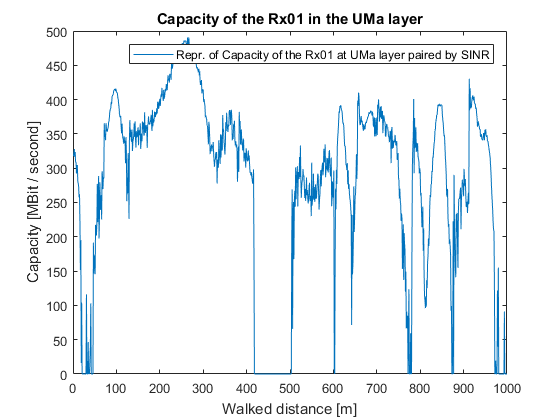
\includegraphics[width=0.8\linewidth]{imagenes/6_3_capacidad_uma_minimo.png}
	\caption{Capacidad del receptor en la capa de macro-celda con una frecuencia baja.}
	\label{fig:simulacion_freq_min_uma}
\end{figure}

\begin{figure}[h!]
	\centering
    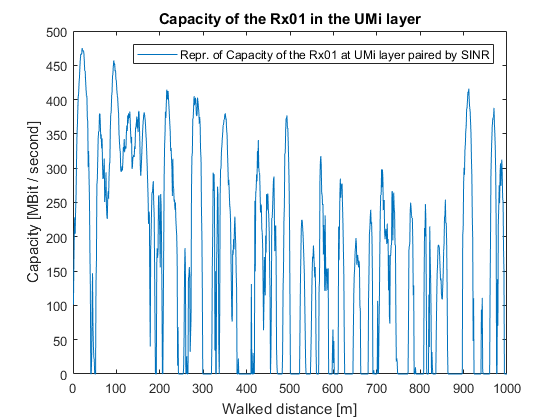
\includegraphics[width=0.8\linewidth]{imagenes/6_3_capacidad_umi_minimo.png}
	\caption{Capacidad del receptor en la capa de micro-celda con una frecuencia baja.}
	\label{fig:simulacion_freq_min_umi}
\end{figure}

En las gráficas resultantes por parte de esta simulación se aprecian unos valores aceptables para la capacidad asignada en la capa de macro-celdas, con picos de aproximadamente 450 Bit/s a pesar de haber algún tramo sin cobertura, mientras que para la simulación de la capa de micro-celdas, aunque el valor máximo se asemeja, existen numerosos tramos en los que no existe cobertura y la capacidad, por tanto, es nula. Esto puede deberse a la proximidad de las celdas y su baja frecuencia. Al bajar la frecuencia, el desvanecimiento de la señal por propagación es menor, lo que conlleva que haya una mayor cantidad de interferencias que limitan el rendimiento de la red.

Acto seguido, se realiza la misma simulación, esta vez modificando las frecuencias de la estaciones base a valores de 2,6 GHz para el caso de las macro-celdas y a 20 GHz para el caso de las micro-celdas. Estas suposiciones resultan lo más cercano al estándar. Los resultados son visibles en las Figuras \ref{fig:simulacion_freq_med_uma} y \ref{fig:simulacion_freq_med_umi}.

Esta simulación ha tomado un total de 20 minutos y 26 segundos para su ejecución, obteniendo un pico de utilización de memoria de 1 GB y ocupando 7,88 MB de almacenamiento al ser guardada en el disco duro.

\begin{figure}[h!]
	\centering
    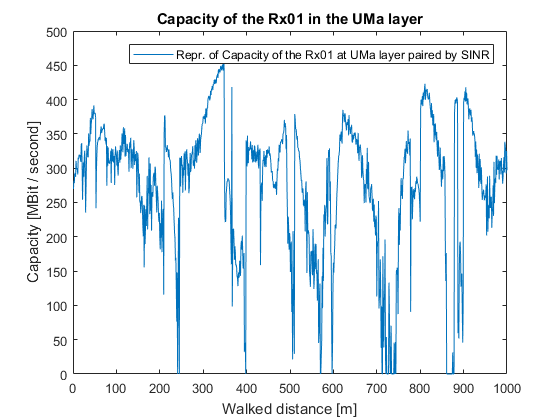
\includegraphics[width=0.8\linewidth]{imagenes/6_3_capacidad_uma_medio.png}
	\caption{Capacidad del receptor en la capa de macro-celda con una frecuencia media.}
	\label{fig:simulacion_freq_med_uma}
\end{figure}

\begin{figure}[h!]
	\centering
    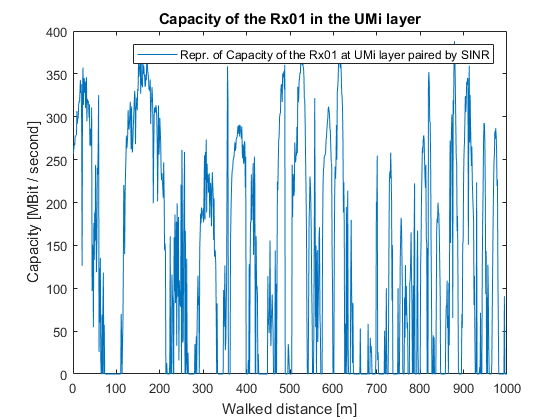
\includegraphics[width=0.8\linewidth]{imagenes/6_3_capacidad_umi_medio.png}
	\caption{Capacidad del receptor en la capa de micro-celda con una frecuencia media.}
	\label{fig:simulacion_freq_med_umi}
\end{figure}

En este caso, la situación para la capa de macro-celdas no varía sustancialmente, viéndose reducida la capacidad asignada a costa de una conexión más estable. Por otro lado, para las micro-celdas, existen tramos con mejor cobertura que en la anterior simulación, aunque sigue siendo muy inestable con tramos de cobertura nula que se podrían justificar por encontrarse en la frontera entre dos celdas.

Para finalizar, se simula un último escenario, esta vez incrementando las frecuencias sustancialmente. Para el caso de la capa de macro-celdas, se ha elegido una frecuencia central de 10 GHz mientras que para la capa de micro-celdas, se ha establecido la frecuencia a 60 GHz. La representación de la capacidad para el receptor en cada caso puede consultarse en las Figuras \ref{fig:simulacion_freq_max_uma} y \ref{fig:simulacion_freq_max_umi}, respectivamente.

Esta simulación ha tomado un total de 20 minutos y 18 segundos para su ejecución, obteniendo un pico de utilización de memoria de 1 GB y ocupando 7,88 MB de almacenamiento al ser guardada en el disco duro.

\begin{figure}[h!]
	\centering
    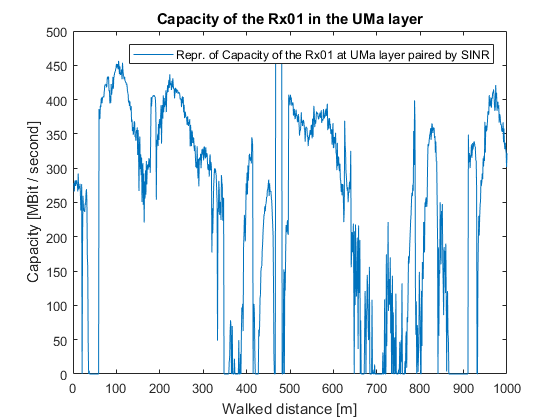
\includegraphics[width=0.8\linewidth]{imagenes/6_3_capacidad_uma_maximo.png}
	\caption{Capacidad del receptor en la capa de macro-celda con una frecuencia alta.}
	\label{fig:simulacion_freq_max_uma}
\end{figure}

\begin{figure}[h!]
	\centering
    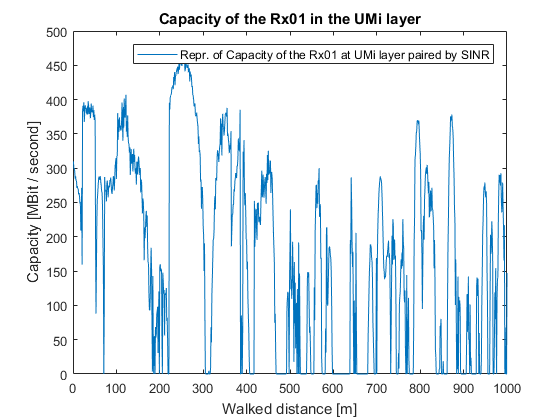
\includegraphics[width=0.8\linewidth]{imagenes/6_3_capacidad_umi_maximo.png}
	\caption{Capacidad del receptor en la capa de micro-celda con una frecuencia alta.}
	\label{fig:simulacion_freq_max_umi}
\end{figure}

Para esta última simulación, la cobertura se ve ligeramente reducida para el caso de la macro-celda, mientras que resulta que para la capa de micro-celda, la cobertura se ve beneficiada y la capacidad aumenta con respecto a simulaciones de menor frecuencia, probablemente por el hecho de recibir menor cantidad de interferencias gracias al desvanecimiento.

Por tanto, se puede concluir que para este escenario en concreto, la configuración óptima sería asignar una frecuencia de 2,6 GHz a la capa de macro-celdas y de 60 GHz a la capa de micro-celdas.

Sin embargo, la principal ventaja de elevar la frecuencia es la de poder ampliar el ancho de banda, característica que no está modelada en este estudio debido a que la implementación del ancho de banda no se ha tenido en cuenta para ser independiente en el caso de macro-celdas y micro-celdas.

Por ello, es de esperar que a medida que se eleva la frecuencia, el ancho de banda asignado también crezca, de modo que, consecuentemente, la capacidad de canal se vea significativamente aumentada.

\subsection{Evolución de la potencia de transmisión}

El siguiente parámetro a evaluar es la potencia de transmisión. Este parámetro influye en la señal recibida, tanto para la estación base conectada como para el resto de estaciones base que interfieren. Por ello, el estudio de cómo afecta la potencia al escenario puede resultar relevante para extraer datos sobre qué potencia de transmisión es la óptima para evitar interferencias a la vez que se recibe una buena calidad de señal.

Para el experimento, se han establecido tres simulaciones que tienen como parámetros comunes la cantidad de celdas, 7 macro-celdas y 19 micro-celdas en concreto, con frecuencias de trabajo de 2,6 GHz y 20 GHz respectivamente y una separación entre centros de 5 km y 2,2 km. El usuario realiza el mismo recorrido que en las anteriores simulaciones y se ha mantenido el ruido fijo con una densidad espectral de potencia de $4,04·10^{-21}$ W/Hz, y un ancho de banda de 100 MHz para ambas capas.

La primera simulación se ha realizado con una potencia de transmisión de 27 dBm para las macro-celdas y de 20 dBm para el caso de las micro-celdas. Se ha representado gráficamente la capacidad del usuario a lo largo de su recorrido, en ambas capas de simulación, que pueden verse en las Figuras \ref{fig:simulacion_pot_min_uma} y \ref{fig:simulacion_pot_min_umi}.

Esta simulación ha tomado un total de 20 minutos y 25 segundos para su ejecución, obteniendo un pico de utilización de memoria de 1 GB y ocupando 7,88 MB de almacenamiento al ser guardada en el disco duro.

\begin{figure}[h!]
	\centering
    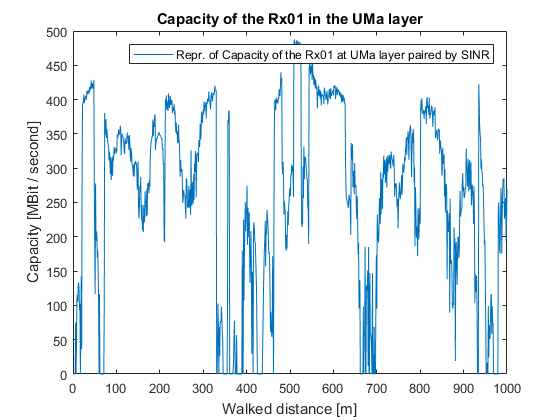
\includegraphics[width=0.8\linewidth]{imagenes/6_4_capacidad_uma_minimo.png}
	\caption{Capacidad del receptor en la capa de macro-celda con una potencia de transmisión baja.}
	\label{fig:simulacion_pot_min_uma}
\end{figure}

\begin{figure}[h!]
	\centering
    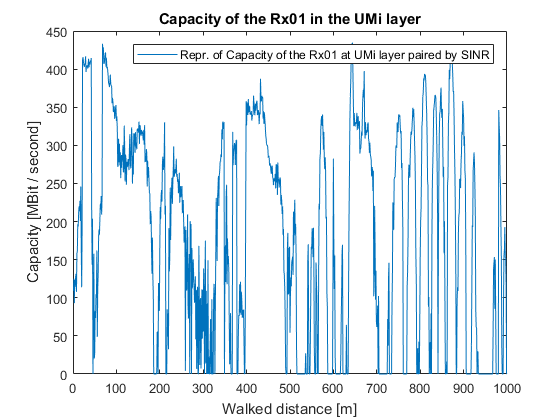
\includegraphics[width=0.8\linewidth]{imagenes/6_4_capacidad_umi_minimo.png}
	\caption{Capacidad del receptor en la capa de micro-celda con una potencia de transmisión baja.}
	\label{fig:simulacion_pot_min_umi}
\end{figure}

Se puede considerar que la estabilidad de la red es aceptable aunque no es la óptima, puesto que la capacidad de red no llega a valores máximos que en otros anteriores escenarios se alcanzaban. Existen algunas zonas sin cobertura, especialmente para la capa de micro-celdas.

Se repite el proceso, esta vez modificando los valores de potencia de transmisión a 40 dBm para macro-celdas y 27 dBm para micro-celdas, obteniendo unos resultados similares a los de la anterior sub-sección, puesto que son los datos estándar, dichos resultados aparecen en la Figura \ref{fig:simulacion_pot_med_uma} y en la Figura \ref{fig:simulacion_pot_med_umi}.

Esta simulación ha tomado un tiempo de ejecución de 21 minutos y 12 segundos, con una ocupación máxima de 1 GB de memoria RAM.

\begin{figure}[h!]
	\centering
    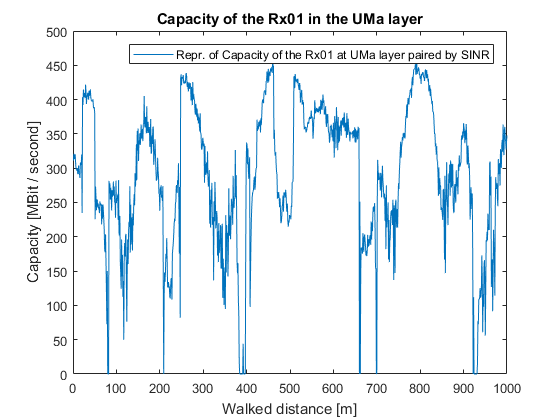
\includegraphics[width=0.8\linewidth]{imagenes/6_4_capacidad_uma_medio.png}
	\caption{Capacidad del receptor en la capa de macro-celda con una potencia de transmisión media.}
	\label{fig:simulacion_pot_med_uma}
\end{figure}

\begin{figure}[h!]
	\centering
    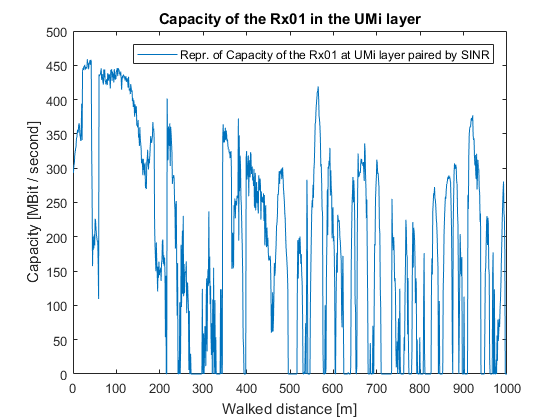
\includegraphics[width=0.8\linewidth]{imagenes/6_4_capacidad_umi_medio.png}
	\caption{Capacidad del receptor en la capa de micro-celda con una potencia de transmisión media.}
	\label{fig:simulacion_pot_med_umi}
\end{figure}

En este caso, el receptor recibe señal aceptable por parte de la capa de macro-celdas, viéndose reducido el tiempo sin conexión con respecto al anterior caso. Por otro lado, la capacidad de la capa de micro-celdas aumenta considerablemente, aumentando ligeramente el tiempo con suficiente cobertura.

Por último, se incrementa la potencia de transmisión a valores de 40 dBm para micro-celdas y 50 dBm para macro-celdas, lo cual resulta sustancialmente mayor de lo que se suele establecer en casos reales. Esta simulación tomó un tiempo de ejecución de 22 minutos y 37 segundos, y sus resultados pueden verse en las Figuras \ref{fig:simulacion_pot_max_uma} y \ref{fig:simulacion_pot_max_umi}.

\begin{figure}[h!]
	\centering
    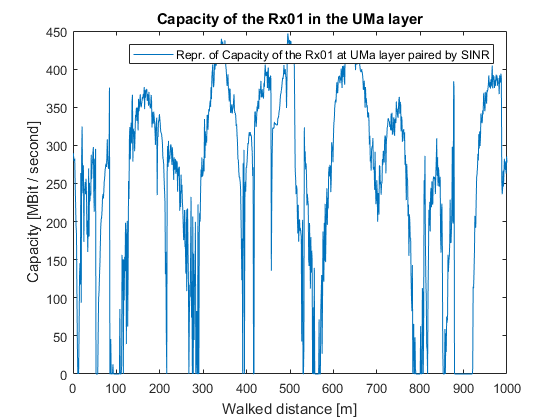
\includegraphics[width=0.8\linewidth]{imagenes/6_4_capacidad_uma_max.png}
	\caption{Capacidad del receptor en la capa de macro-celda con una potencia de transmisión alta.}
	\label{fig:simulacion_pot_max_uma}
\end{figure}

\begin{figure}[h!]
	\centering
    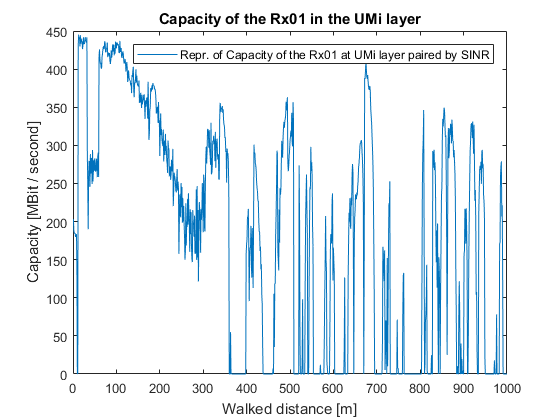
\includegraphics[width=0.8\linewidth]{imagenes/6_4_capacidad_umi_max.png}
	\caption{Capacidad del receptor en la capa de micro-celda con una potencia de transmisión alta.}
	\label{fig:simulacion_pot_max_umi}
\end{figure}

Para el enlace con la macro-celda asociada, los tramos sin suficiente cobertura se ven ligeramente incrementados, a la vez que la capacidad media se ve reducida. Esta es una prueba directa de que la potencia de transmisión puede ser contraproducente en cuanto a interferencias se refiere.

Por otro lado, el enlace de micro-celdas se ve beneficiado con un incremento del tiempo de cobertura aceptable, disminuyendo zonas sin conexión, Sin embargo, este resultado no puede ser concluyente ni debe ser interpretado como una consecuencia directa de incrementar la potencia, puesto que el usuario se encuentra en el filo de las celdas de micro-celda, por lo que al aumentar la potencia, se mejoran las condiciones en esas situaciones, mientras que en situaciones más cercanas al centro de la celda, el rendimiento será menor debido a que las demás celdas interferirán con esa señal.

\subsection{Evolución de la separación geográfica}

Como última serie de experimentos, se ha diseñado un último conjunto de simulaciones en el que se estudia cómo afecta el tamaño de las celdas en el rendimiento de la red. Para ello, se realizarán tres simulaciones distintas donde se varía la distancia entre los centros de las celdas.

La simulación se ha establecido con unos parámetros estándar de 7 macro-celdas y 19 micro-celdas, con 40 dBm de potencia de transmisión y 2,6 GHz de frecuencia para macro-celdas y 27 dBm de potencia y 20 GHz de frecuencia para micro-celdas.

En la primera simulación se ha elegido una separación entre los centros de macro-celdas de 600 m, mientras que para los centros de micro-celdas se ha establecido una separación de 200 m. Esta simulación ha tomado 21 minutos y 8 segundos para su ejecución y pueden verse sus resultados en la Figura \ref{fig:simulacion_sep_min_uma} y en la Figura \ref{fig:simulacion_sep_min_umi}, donde está representada la capacidad del receptor para ambos casos.

\begin{figure}[h!]
	\centering
    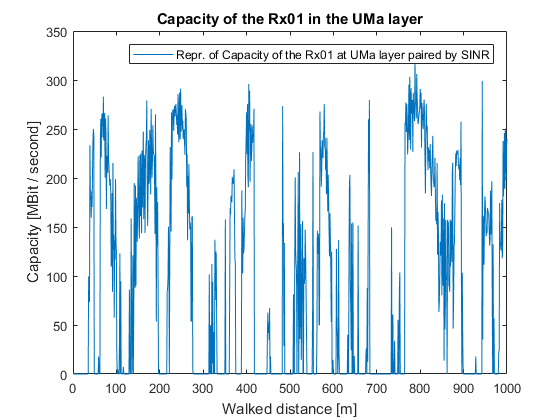
\includegraphics[width=0.8\linewidth]{imagenes/6_5_capacidad_uma_min.png}
	\caption{Capacidad del receptor en la capa de macro-celda con un tamaño de celdas mínimo.}
	\label{fig:simulacion_sep_min_uma}
\end{figure}

\begin{figure}[h!]
	\centering
    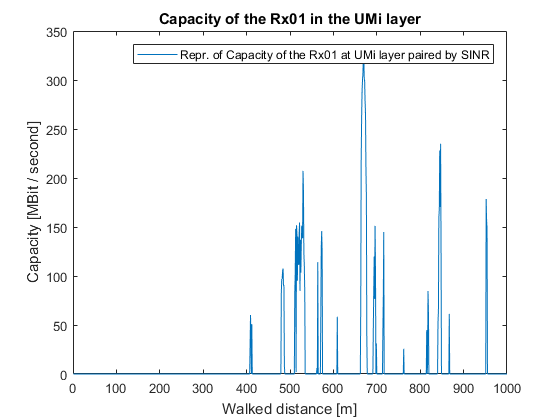
\includegraphics[width=0.8\linewidth]{imagenes/6_5_capacidad_umi_min.png}
	\caption{Capacidad del receptor en la capa de micro-celda con un tamaño de celdas mínimo.}
	\label{fig:simulacion_sep_min_umi}
\end{figure}

En ambos resultados se aprecia un rendimiento pésimo por parte de la red, con valores máximos de capacidad de apenas 200 Mbit/s en macro-celdas, cuando la media en el resto de simulaciones había resultado en 500 Mbit/s. La zona de cobertura se ve reducida en comparación de igual modo.

En cuanto a micro-celdas, la cobertura, aun estando el receptor emparejado a la estación base de mayor SINR, es prácticamente nula, imposibilitando el servicio para dicho usuario.

Estos resultados son de esperar debido a la poca separación entre estaciones base que hacen que la interferencia se vea aumentada considerablemente.

Se repite la simulación para una separación de 5 km en macro-celdas y de 2,2 km para micro-celdas, con un tiempo de ejecución de 21 minutos y 7 segundos. Los resultados, que a priori se esperan parecidos a anteriores simulaciones, se representan en las Figuras \ref{fig:simulacion_sep_min_uma} y \ref{fig:simulacion_sep_min_uma}.

\begin{figure}[h!]
	\centering
    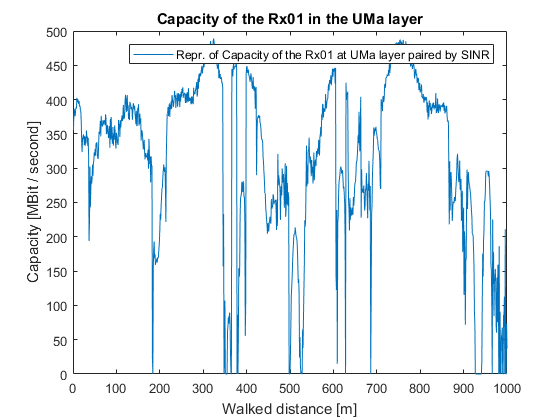
\includegraphics[width=0.8\linewidth]{imagenes/6_5_capacidad_uma_med.png}
	\caption{Capacidad del receptor en la capa de macro-celda con un tamaño de celdas medio.}
	\label{fig:simulacion_sep_med_uma}
\end{figure}

\begin{figure}[h!]
	\centering
    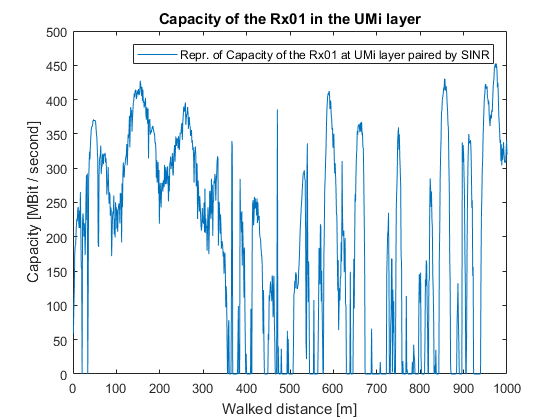
\includegraphics[width=0.8\linewidth]{imagenes/6_5_capacidad_umi_med.png}
	\caption{Capacidad del receptor en la capa de micro-celda con un tamaño de celdas medio.}
	\label{fig:simulacion_sep_med_umi}
\end{figure}

Como se puede observar, las condiciones para este tamaño de celdas se ven sustancialmente mejoradas, con una experiencia de servicio que resultaría satisfactoria para el usuario, ya que contaría con una cobertura estable en todo su recorrido para ambas capas de simulación.

La última simulación se realiza con una separación entre celdas de 11 km para macro-celdas, y 5 km para micro celdas. Esto supone que el escenario de simulación se extienda hasta aproximadamente 440 km$^{2}$, por lo que el kilómetro de la trayectoria del receptor es en proporción un recorrido corto. Los resultados pueden observarse en las Figuras \ref{fig:simulacion_sep_max_uma} y  \ref{fig:simulacion_sep_max_umi}, tomando un tiempo de simulación de 22 minutos y 14 segundos.

\begin{figure}[h!]
	\centering
    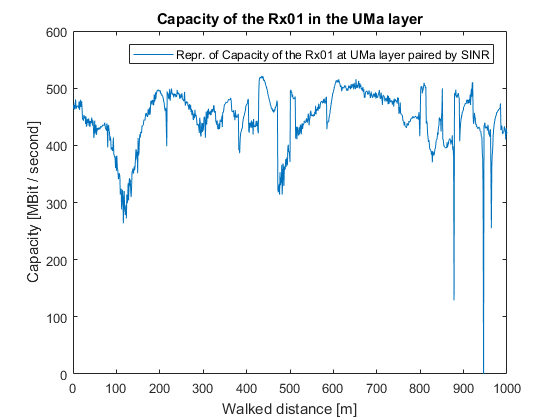
\includegraphics[width=0.8\linewidth]{imagenes/6_5_capacidad_uma_max.png}
	\caption{Capacidad del receptor en la capa de macro-celda con un tamaño de celdas máximo.}
	\label{fig:simulacion_sep_max_uma}
\end{figure}

\begin{figure}[ht!]
	\centering
    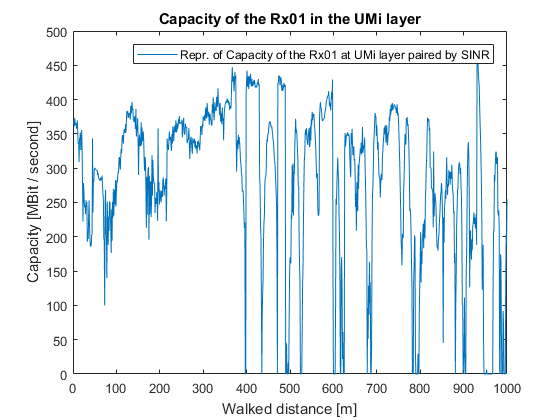
\includegraphics[width=0.8\linewidth]{imagenes/6_5_capacidad_umi_max.png}
	\caption{Capacidad del receptor en la capa de micro-celda con un tamaño de celdas máximo.}
	\label{fig:simulacion_sep_max_umi}
\end{figure}

En esta última ejecución se muestra un rendimiento de la red mayor que en el resto de simulaciones anteriores, con un tiempo de servicio y de cobertura estable de aproximadamente el 100\% en el caso de macro-celda, y muy cercano al total también en micro-celda.

Esto demuestra que el principal problema que afecta al rendimiento de la red son las interferencias, puesto que al alejar la fuente de interferencias del receptor, la capacidad asignada al mismo se ve considerablemente mejorada. En este caso, las mejores condiciones para el escenario son las de aumentar el tamaño de celda para asegurar una mayor cobertura en las mismas sin interferencias.

Los resultados refuerzan la necesidad de incorporar al simulador algún sistema de planificación que implemente reuso de frecuencias, con la finalidad de mejorar el rendimiento de la red y de asemejarse a los sistemas que se utilizan en la actualidad.